\documentclass[10pt]{article}
%\documentclass[review]{siamart1116}
%\documentclass[review]{siamonline1116}

\usepackage{amsmath}
\usepackage{amsfonts}
\usepackage{amssymb}
\usepackage{fancyhdr}
\usepackage[margin=0.75in]{geometry}
\usepackage{graphicx}
\usepackage[section]{placeins}
\usepackage{nicefrac}
\usepackage{bm}
\usepackage{xcolor}
\usepackage[format=plain,indention=.5cm, font={it,small},labelfont=bf]{caption}
\usepackage{subcaption}
\usepackage{float}
\usepackage{enumerate}
\usepackage{tikz}
\usetikzlibrary{arrows.meta}
\usepackage[all]{xy}
\usepackage{url}
\usepackage{multicol}



%%%%%%%%%%%%%%%%%%%%%%%%%%%%%%%%%%%%%%%%%%%%%%%%%%%%%%%%%%%%%%%%%%%%%%%%%%%%%%%%%%%%%%%%%%%%%%%%%%%%%%%%%%%%%%%%%%
\usepackage{stackengine}
\usepackage{amsthm}
\usepackage{cleveref}


\newtheorem{theorem}{Theorem}
\newtheorem*{theorem*}{Theorem}
\newtheorem{lemma}{Lemma}
\newtheorem*{lemma*}{Lemma}
\newtheorem{conj}{Conjecture}
\newtheorem{corollary}{Corollary}
\newtheorem{clm}{Claim}
\newtheorem{rmk}{Remark}
\newtheorem{note}{NOTE}
\newtheorem{method}{Method}

\theoremstyle{definition}
\newtheorem*{def*}{Definition}
\newtheorem{definition}{Definition}
\numberwithin{theorem}{section}
\numberwithin{definition}{section}
\numberwithin{lemma}{section}
\numberwithin{corollary}{section}
\numberwithin{clm}{section}
\numberwithin{rmk}{section}

\newcommand{\low}[1]{$_{\text{#1}}$}
\newcommand\xput[2][0.5]{%
	\rule{#1\linewidth}{0pt}\makebox[0pt][c]{#2}\hfill}

\setlength{\headheight}{15pt}
\pagestyle{fancy}
\renewcommand{\headrulewidth}{0pt}
\fancyhead[L]{Brunner}
\fancyhead[C]{Co-Occurrance Network}
\fancyhead[R]{\today}
\lfoot{}
\cfoot{\thepage}
\rfoot{}

%%%%%%%%%%%%%%%%%%%%%%%%%%%%%%%%%%%%%%%%%%%%%%%%%%%%%%%%%%%%%%%%%%%%%%%%%%%%%%%%%%%%%%%%%%%%%%%%%%%%%%%%%%%%%%%%%%
%
%
%\newsiamthm{clm}{Claim}
%\newsiamremark{rmk}{Remark}
%\newsiamremark{note}{NOTE}
%\numberwithin{theorem}{section}
%
%
%%%%%%%%%%%%%%%%%%%%%%%%%%%%%%%%%%%%%%%%%%%%%%%%%%%%%%%%%%%%%%%%%%%%%%%%%%%%%%%%%%%%%%%%%%%%%%%%%%%%%%%%%%%%%%%%%%
\newenvironment{inbox}[1]
{\begin{center}
		\begin{tabular}{|p{0.9\textwidth}|}
			\hline
			{\bf #1}\\
		}
		{ 
			\\\\\hline
		\end{tabular} 
	\end{center}
}
\newenvironment{inbox2}
{\begin{center}
		\begin{tabular}{|p{0.9\textwidth}|}
			\hline \vspace{-0.5 cm}
		}
		{ 
			\\ \hline
		\end{tabular} 
	\end{center}
}




\newcommand{\nhalf}{\nicefrac{1}{2}}
\newcommand{\eps}{\epsilon_{machine}}
\newcommand{\ol}{\overline}
\renewcommand{\b}{\bm}

\definecolor{dgreen}{RGB}{49,128,23}
\definecolor{lgreen}{RGB}{77, 255, 166}
\definecolor{nicepink}{RGB}{255, 0, 102}
\definecolor{nicered}{RGB}{255, 80, 80}
\definecolor{lblue}{RGB}{102, 163, 255}
\definecolor{lgray}{RGB}{217, 217, 217}

\newcommand{\bE}{\mathbb{E}}
\newcommand{\bP}{\mathbb{P}}
\newcommand{\bR}{\mathbb{R}}
\newcommand{\bN}{\mathbb{N}}
\newcommand{\bZ}{\mathbb{Z}}
\newcommand{\bQ}{\mathbb{Q}}
\newcommand{\bC}{\mathbb{C}}
\newcommand{\cA}{\mathcal{A}}
\newcommand{\cB}{\mathcal{B}}
\newcommand{\cC}{\mathcal{C}}
\newcommand{\cD}{\mathcal{D}}
\newcommand{\cE}{\mathcal{E}}
\newcommand{\cF}{\mathcal{F}}
\newcommand{\cG}{\mathcal{G}}
\newcommand{\cH}{\mathcal{H}}
\newcommand{\cI}{\mathcal{I}}
\newcommand{\cJ}{\mathcal{J}}
\newcommand{\cK}{\mathcal{K}}
\newcommand{\cL}{\mathcal{L}}
\newcommand{\cM}{\mathcal{M}}
\newcommand{\cN}{\mathcal{N}}
\newcommand{\cO}{\mathcal{O}}
\newcommand{\cP}{\mathcal{P}}
\newcommand{\cQ}{\mathcal{Q}}
\newcommand{\cR}{\mathcal{R}}
\newcommand{\cS}{\mathcal{S}}
\newcommand{\cT}{\mathcal{T}}
\newcommand{\cU}{\mathcal{U}}
\newcommand{\cV}{\mathcal{V}}
\newcommand{\cW}{\mathcal{W}}
\newcommand{\cX}{\mathcal{X}}
\newcommand{\cY}{\mathcal{Y}}
\newcommand{\cZ}{\mathcal{Z}}

\newcommand{\inter}{\text{\normalfont int}}
\newcommand{\ka}{\kappa}
\newcommand{\fp}{\varrho}
\newcommand{\problem}[2]{ \ \\ {\bf #1} {\it #2} \ \\} 

\renewcommand{\arraystretch}{1.5}
\renewcommand{\thefootnote}{\fnsymbol{footnote}}	
\author{Jim Brunner}
\title{Using a co-occurrance network}

\begin{document}
\maketitle
\section{Network Building}
My project centered around the creation and analysis of ecological networks of microbiomes. I built networks, in the form of graphs $\cG = (\cV, \cE)$, based on co-occurrence of organisms at various taxonomic levels. In these graphs, vertices are labeled by taxa name, and edge sets are defined by co-occurrence or correlation. This project is meant to support the EDGE bioinformatics platform \cite{edge}. 

\subsection{Co-occurrence construction}
One method of building a co-occurrence network from a set of samples of microbial communities is to simply count how often various microbes co-occur. This will be referred to as the ``binning method". 

Given a set of samples with abundances of organisms, we map the abundances to discrete levels, as proportions of the maximum abundance \emph{of that organism}. Precisely, let the samples be $s_j$ and raw abundance of organism $i$ in sample $i$ be $r_{ij}$. we map the abundances according to
\[
a(r_{ij})  = \left\{
\begin{array}{c c}
\lfloor\left(\frac{r_{ij}}{\max_{s_k}(r_{ik})}\right) n \rfloor + 1 &  \frac{r_{ij}}{\max_{s_k}(r_{ik})} \geq m \\
0 & \frac{r_{ij}}{\max_{s_k}(r_{ik})} < m
\end{array}
\right.
\]
where $m$ is some minimum. Then, we create weighted edges between vertices (where $0$ weight means no edge exists) where the weights of edges in $\cE^*$ are
\[
w^*_{ik} = \frac{\|\{i: a(r_{ij}) = a(r_{kj}) \neq 0\} \|}{S}
\]
Here, $S$ is the total number of samples. That is, $w^*_{ik}$ is a count the proportion of samples in which the two taxa appear at the same discretized level. 

Next, I account for random coincidence of taxa in a sample, following \cite{coocc}. To do this, I compare to a null model. The null model is defined in the following way.
\[
A_i= \sum_{s_j} \b{1}_{a(r_{ij}) \neq 0}
\] 
and 
\[
S_j^l  = \sum_{v_i} \b{1}_{a(r_{ij}) = l}
\]
Then, the null model assumes that if
\[
X_{ijl} \sim \mathit{binom}\left(A_i, \frac{S_j^l}{\sum_{jl} S_j^l}\right)
\]
then $P(a_{ij}^{null} = l) = 1-P(X_{ijl} = 0)$. This allows us to calculate the probability of co-occurrence of taxa under the null model. Let $w_{ik}^{null}$ be
\[
w^{null}_{ik} = \|\{i: a_{ij}^{null} = a_{kj}^{null} \neq 0\} \|
\]
Then,
\[
P(w_{ik}^{null} = K) =  \sum_{\{A \subset \cV_2:|A| = k\}} \prod_{l\in A} a_{il}a_{kl}\prod_{l \not\in A} (1- a_{il}a_{kl})
\]
Ideally, the weights $\cE$ would be defined by
\[
w_{ik} = \left\{ \begin{array}{c c}
w_{ik}^* & P(w_{ik}^{null} \geq w_{ik}^*) \leq 0.05\\
0 & P(w_{ik}^{null} < w_{ik}^*) > 0.05
\end{array}\right.
\]
However, that probability is intractable to compute. Instead, let
\[
\widetilde{P}(w_{ik}^{null} = K) = \sum_{l=0}^i \binom{N_1}{l}\binom{N_2}{K-l} p_1^j p_2^{K-l} (1-p_1)^{N-l}(1-p_2)^{N-K+l}
\]
where
\[
p_1 = p_a - \left(\frac{N_2}{N_1}\frac{N(\mu-\sigma^2)- \mu^2}{N^2}\right)^{\nhalf}
\]
and 
\[
p_2 = p_a - \left(\frac{N_1}{N_2}\frac{N(\mu-\sigma^2)- \mu^2}{N^2}\right)^{\nhalf}
\]
Finally, $N_1$, $N_2$ are to ensure that $p_1,p_2 \in [0,1]$. These must satisfy:
\[
\frac{\mu N (1-p_a) - N\sigma^2}{N(1-p_a)- \sigma^2} \leq N_2 \leq \frac{\mu^2}{\mu- \sigma^2}
\]
with $\mu$ the mean of the real distribution, $\sigma^2$ the variance, and $p_a = \frac{1}{S}\sum_{i} a_{ij}a_{kj}$. So, I take 
\[
w_{jk} = \left\{ \begin{array}{c c}
w_{ik}^* & \widetilde{P}(w_{jk}^{null} \geq w_{ik}^*) \geq t\\
0 & \widetilde{P}(w_{jk}^{null} < w_{ik}^*) > t
\end{array}\right.
\]

\subsection{Correlation construction}
An alternative to the binning above is sample correlation, as in \cite{gut}. With $N$ samples, that is:
\[
\rho_{xy} = \frac{1}{N}\frac{(\b{x}- \mu_x\b{1}) \cdot (\b{y} - \mu_y\b{1})}{\sigma_x \sigma_y}
\]
where $\mu_x$ is the mean abundance of taxa $x$, and $\sigma_x$ is the standard deviation of abundance of taxa $x$ across samples. This can be constructed by modifying the data matrix and then multiplying with it's transpose, making it much faster to compute than the binning method. In expectation, this the co-variance divided by the product of the variances. I then construct a graph with weighted edges
\[
w_{ik} = \left\{\begin{array}{c c}
\rho_{\b{r}_i\b{r}_k} & \rho_{\b{r}_i\b{r}_k}\geq 0.8\\
0 &  \rho_{\b{r}_i\b{r}_k}< 0.8
\end{array}\right.
\]

Alternatively, I can first ``thresh-hold" the abundances given, converting to binary presence/absence data. To do this, I find the mean of all non-zero abundance values $\mu_{nz}$, and then
\[
r^*_{ij} = \left\{\begin{array}{c c}
1 & r_{ij} \geq 0.01\mu_{nz}\\
0 & r_{ij} < 0.01 \mu_{nz}
\end{array}\right.
\]
The network is then constructed using sample correlation just as before.

Again, I check the significance of each edge, removing edges that have a high probability of occurring in a null model. I check this using Monte-Carlo simulation by estimating $p_{ik} \approx P(\rho_{\b{r}_i^{null}\b{r}_k^{null}} > \rho_{\b{r}_i\b{r}_k})$. I take enough Monte-Carlo trials for a $95\%$ confidence interval of length $0.03$. I then adjust edges so that
\[
p_{ik} > 0.05 \Rightarrow w_{ik} = 0
\]

\begin{inbox}{The Null Model}
	Rather than simply generate an Erd\H{o}s-R\'{e}nyi random graph with some chosen parameter, I generate a graph that more closely reflects the idea of random data. That is, I start with random data and then generate a graph. I generate random data in the following way. Let 
	\[
	N_j = |\{i: r_{ij} \neq 0\}|
	\]
	and 
	\[
	P_i = \frac{|\{j: r_{ij}\neq 0 \}|}{|\{(i,j): r_{ij}\neq 0 \}|}
	\]
	then I take 
	\[
	\hat{r}_{ij} = \mathit{binom}(N_j,P_i)
	\]
	as randomly generated abundance data. The values $N_i$ are the counts of appearances of taxi $i$, while the values $P_j$ are the proportions of all appearances which happen within each sample. 
	
	Then, I construct our random graph from this random data. If $\hat{\b{r}}_i$ is the vector of random ``abundances" of taxa $i$, I have edges
	\[
	w_{ik}^{null} = \frac{1}{N}\frac{(\b{\hat{\b{r}}_i}- \hat{\mu}_i\b{1}) \cdot (\hat{\b{r}}_k - \hat{\mu}_k\b{1})}{\hat{\sigma}_i \hat{\sigma}_k}
	\]
\end{inbox}

The null model's use of a binomial random variable can be interpreted in the following way. A ``success" for a taxa/sample pair is an appearance of the taxa in the sample. The number of trials is the number of times the taxa appears in the data set. The probability of success is the proportion of all appearances which happen within the sample. This does have some drawbacks: notably that it does not preserve total abundance, or even total appearances. It allows more than one ``success" for a single taxa/sample pair, which could be interpreted as higher abundance. Our ``random samples" should be scaled by average abundances of a taxa across samples to ``look like" real data. This doesn't effect correlation, because $\mathit{Cov}(ax,by) = ab\mathit{Cov}(x,y)$, and $\sigma_x = \mathit{Cov}(x,x)^{\nhalf}$, implying that $w_{ik} = \mathit{Cor}(\hat{\b{r}}_i,\hat{\b{r}}_k) =  \mathit{Cor}(a\hat{\b{r}}_i,b\hat{\b{r}}_k)$. Notice also that the null model is the same as in the binning procedure, with a different construction of a correlation graph.

In \cite{coocc}, this model is called the ``binomial model". Interestingly, that paper argues that an ``edge swapping" model is more accurate. A random permutation of the data also used in \cite{gut}. However, I have chosen the binomial model for speed.

\subsection{Significance of the network}
The networks connected by the methods above would not occur in randomized data, and so there is some significance to these networks. I generate random data as in the correlation construction of the network. I then use Monte-Carlo simulation to estimate the following
\begin{itemize}
	\item $P(\mu_d < \mu_d^{null})$, where $\mu_d$ is the mean degree of the nodes of a network
	\item $P(\sigma_d < \sigma_d^{null})$, where $\sigma_d$ is the variance of degrees of the nodes of a network
	\item $P(\lambda_{max} < \lambda_{max}^{null})$, where $\lambda_{max}$ is the largest eigenvalue of the adjacency matrix
	\item $P(\lambda_{min} < \lambda_{min}^{null})$, where $\lambda_{min}$ is the smallest eigenvalue of the adjacency matrix
	\item $P(|\cE| < |\cE^{null}|)$
\end{itemize} 

The result with $10,000$ Monte Carlo trials was that it was extremely rare for a network constructed from a null model to have higher mean degree, higher degree variance, larger maximum eigenvalue, smaller minimum eigenvalue, or more edges. This suggests that the networks constructed from real data would be very unexpected according to the null model. 

In addition to testing the complete network, I performed the same analysis on networks built from randomly drawn subsets of the data.

\begin{figure}
	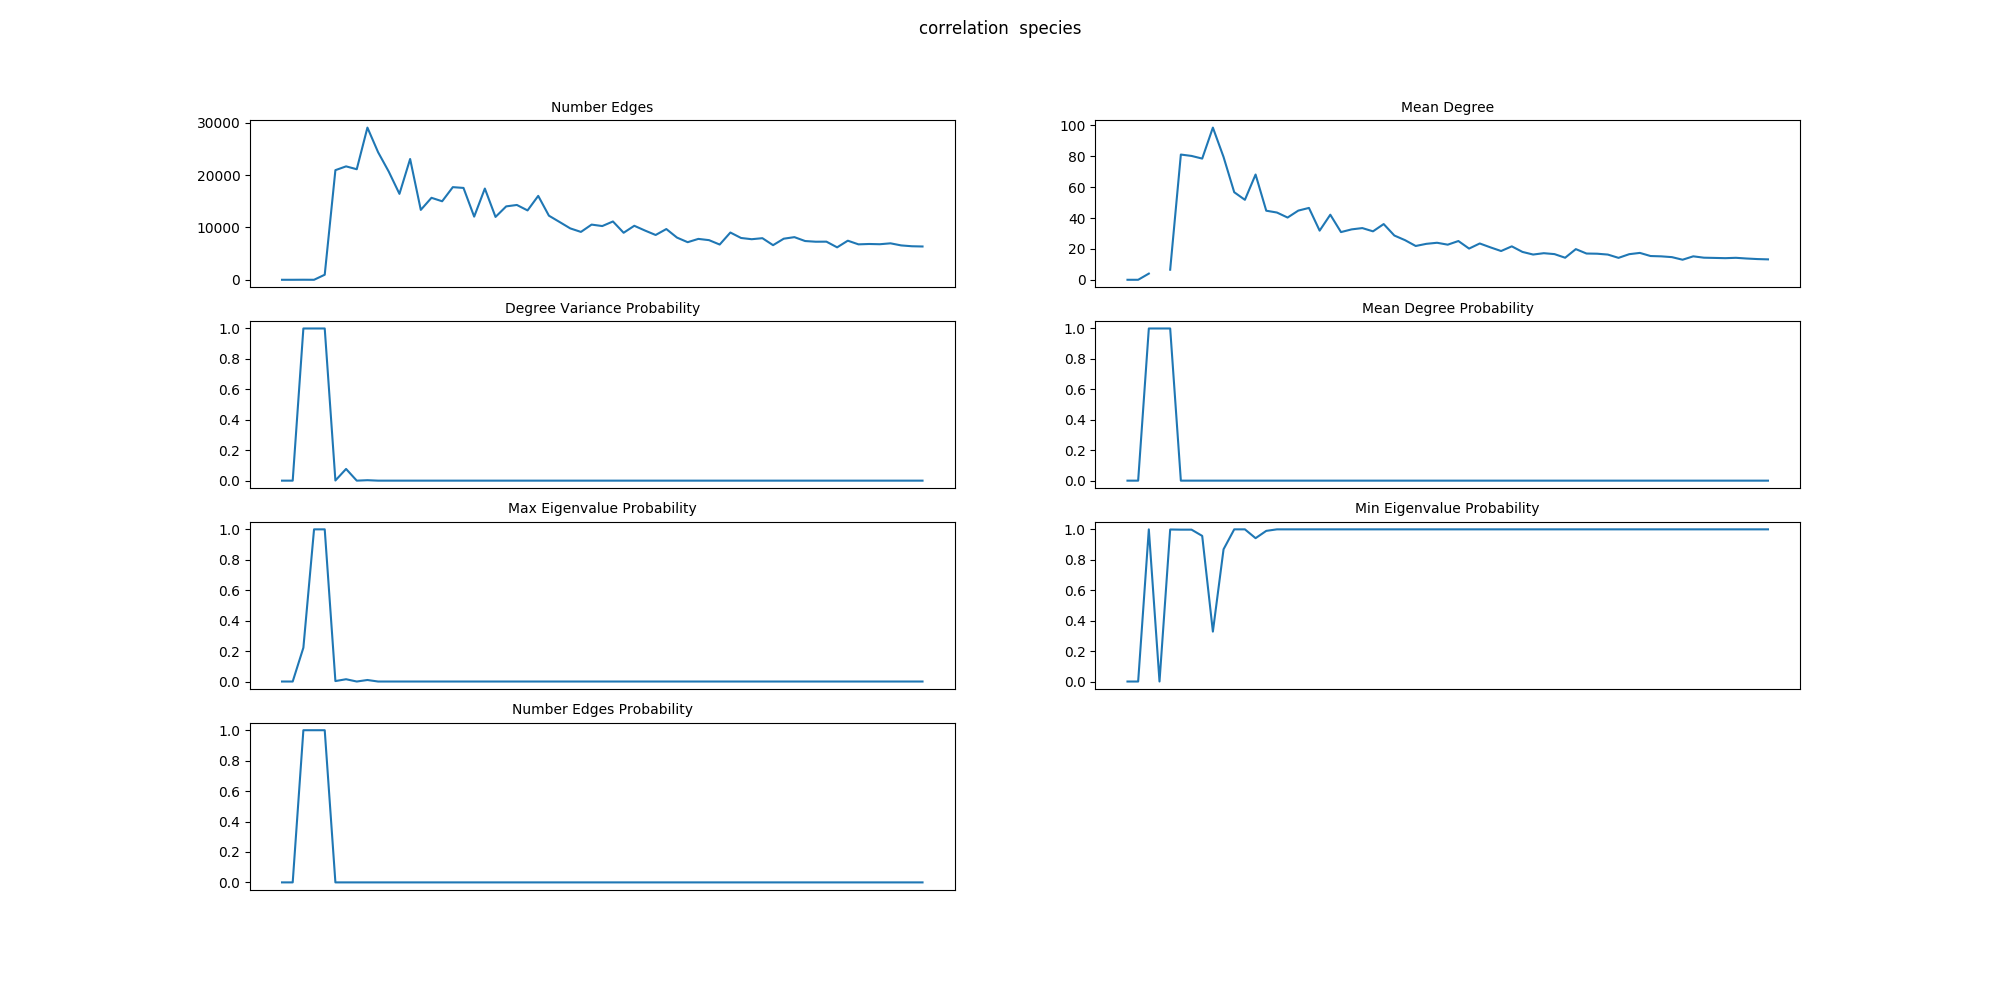
\includegraphics[scale = 0.4]{../stat_figs/pears_1000__species.png}
	\caption{The result of Monte-Carlo estimation of the likelihood of various network statistics, as well as the number of edges and mean degree. The networks were made from correlations using randomly drawn subsets of increasing size of the data at the species level, from 1 sample to all 60 samples. For each network, 1000 random trials were generated according to the above null model in order to estimate likelihood of statistics.}\label{montecarlos}
\end{figure}

This analysis is computationally difficult. In order to estimate how it scales with number of samples, I recorded the time for the Monte Carlo estimation, using randomly drawn subsets of the data. It appears that if $n$ is the number of samples and $\tau$ the time to compute, then $\tau \approx \frac{1}{3} n$ seconds for samples with $\sim 250$ taxa. 

\section{Networks Built}

To test the ideas of this paper, we used HMP data to build networks. We built ``full" networks using about 1300 individual samples. We also used 300 test samples (not used in the construction of the network), randomly chosen from the data set (uniformly, ignoring metadata), to test various network analysis ideas. In addition to the full network, we built networks using subsets of the data corresponding the available metadata, which was the sample's origin in the human body. We therefore built, in addition to the full network, networks corresponding to samples labeled:
\begin{multicols}{2}
\begin{itemize}
	\item Anterior Nares
	\item Attached
	\item Buccal Mucosa
	\item Hard Palate
	\item Keratinized Gingiva
	\item L Retroauricular Crease
	\item Mid Vagina
	\item Palatine Tonsils
	\item Posterior Fornix
	\item R Retroauricular Crease
	\item Saliva
	\item Stool
	\item Subgingival Plaque
	\item Supragingival Plaque
	\item Throat
	\item Tongue Dorsum
	\item Vaginal Introitus
\end{itemize}
\end{multicols}
\section{Network Analysis}
Network clustering identifies related nodes in a graph. This can be used in combination with sample metadata to help find characteristics that effect the microbial community in a sample. Sample metadata can be associated to nodes of a network by the frequency with which a taxa appears along with some sample characteristic. For a metadata category  $C$ that allows a discrete set of $m$ characteristics $c_i$, let
\[
r_i^{c_k} = \sum_{j:s_j \text{ has } c_k} r_{ij}
\]
Let $\mu_i^C$ be the mean of $\{r_i^{c_l}\}_{l=1}^m$, and $\sigma_i^C$ the variance. Then, taxa $i$ is assigned to $c_k$ if
\[
r_i^{c_k} > \mu_i^C + 1.5\sigma_i^C
\]

Community clustering minimizes a function of the graph called modularity \cite{PhysRevE.70.066111}\cite{PhysRevE.70.056131}. That is 
\[
Q = \frac{1}{2m}\sum_{i,j}\left(w_{ij} + \frac{d_id_j}{2m}\right) \delta(c_i,c_j)
\]
where $m = \sum_{i\sim j} w_{ij}$, $d_i$ is the (weighted) degree of vertex $i$, $c_i$ is the community containing vertex $i$, and $\delta$ is the Kronecker $\delta$. This done by a gradient search/greedy algorithm.

Spectral clustering performs a $k$-means clustering on the rows of the matrix whose columns are the $k$ eigenvectors of the graph Laplacian corresponding to the smallest $k$ eigenvalues \cite{vonLuxburg2007} . Intuitively, this means it clusters points together that are close in the first $k$ (slowest decaying) modes of the diffusion equation on the graph. 

I characterized nodes according to where the sample was taken from a human body, and used Cytoscape \cite{cyotscape} to visualize the connection between this classification and the two clustering methods.

\begin{figure}
	\begin{center}
		\begin{subfigure}[b]{0.48\linewidth}
			\begin{center}
				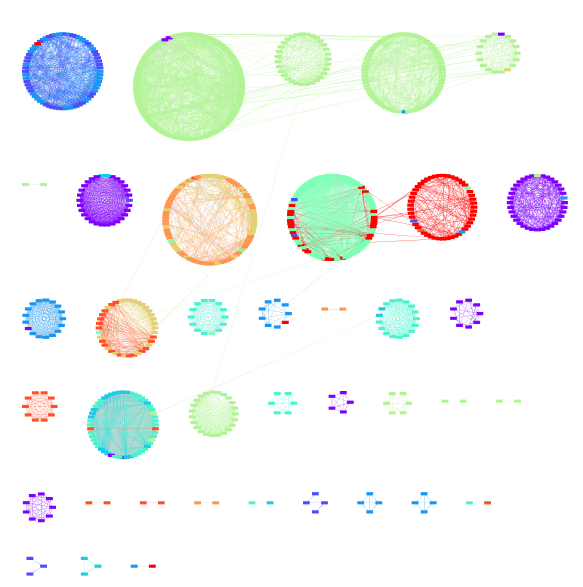
\includegraphics[scale = 0.3]{comm_samp.png}	
			\end{center}
			\caption{Community clustering.}
		\end{subfigure}
		\begin{subfigure}[b]{0.48\linewidth}
			\begin{center}
				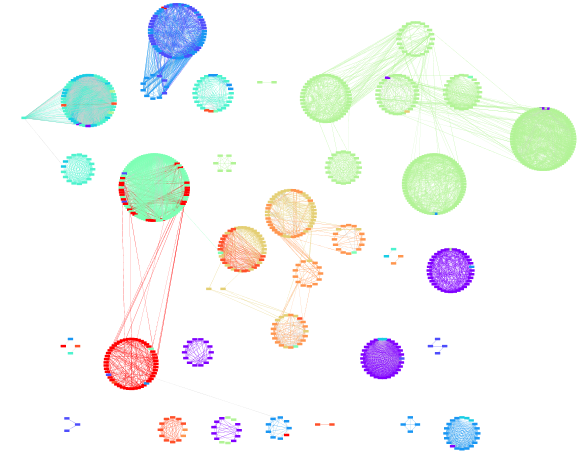
\includegraphics[scale = 0.35]{spect_sample.png}	
			\end{center}
			\caption{Spectral clustering.}
		\end{subfigure}
		\caption{Clustering of the correlation network using two methods compared to classification by sample metadata (location). Colors represent sample metadata. Nodes are grouped in circles by cluster.}\label{cluster}
	\end{center}
\end{figure}

\section{Using the network to analyze a sample}

Ideally, co-occurrence and correlation networks could be used to analyze GOTTCHA results, to assess the probability that the set of taxa identified by GOTTCHA would occur together. Assume that the probability that any vertex pair occurs together is the edge weight between the nodes representing the two taxa. Precisely, assume that
\[
w_{ik} = P(i \, \&\, k \in  s_i)
\]
where $s_j$ is sample $j$. 

Consider the simplest case of thresholded abundance. Assume GOTTCHA found taxa $a,b,c,...,n$. The first thing we might want to know is
\[
P(a | b,c,d,...,n), \, P(b|a,c,d,...,n) ,\, \mathit{etc}
\]
By assumption, edge weights and frequency counts of individual taxa can be used to determine pairwise conditional probabilities. We can also bound triplets (assuming $P(c,b) \neq 0$):
\[
P(a|b,c) \leq \frac{\min_{(i,j) \subset \{a,b,c\}}(P(i,j))}{P(b,c)}
\]
but we can't do any better than triplets explicitly, because we don't have any sort of independence (conditional or otherwise) and because our network is not acyclic. 

We can consider the network a Markov random field \cite{machine_learning}. This can give us a way to calculate the probability a group of taxa occurs together. The main idea of a MRF is that nodes are conditionally independent of nodes they aren't neighbors of (conditioned on ones they are neighbors of). If $c$ are the (maximal) cliques of the graph (complete sub-graphs), then the probability of configuration $\b{x}$ is
\[
P(\b{x}) = \frac{1}{Z} \prod_{c} \psi_c (x_{c})
\]	
where $Z$ is a normalizing constant and $\psi_c$ are some functions, often called ``potential functions"\cite{machine_learning}. If we have a sample that contains the subset $\b{s}$, we can calculate something. Let $C_s$ be the cliques represented in $\b{s}$.
\[
P(\b{s}) = \frac{1}{Z}\sum_{\{\b{x} : s\subset \b{x}\}}\prod_{c\in C_s}\psi_c(\b{x})
\]
And we can ignore cliques not represented in $\b{s}$. The difficulty in this approach is to determine the functions $\psi_c$.

\subsection{Determining $\psi_c$}

Before determining $\psi_c$, it should be noted that we have a choice of configuration space of the network. We can use a binary $\{1,0\}^N$ space to denote presence or absence, or we can choose a continuous space to include abundances. To begin, I will only consider presence \& absence.

\begin{figure}
	\begin{center}
		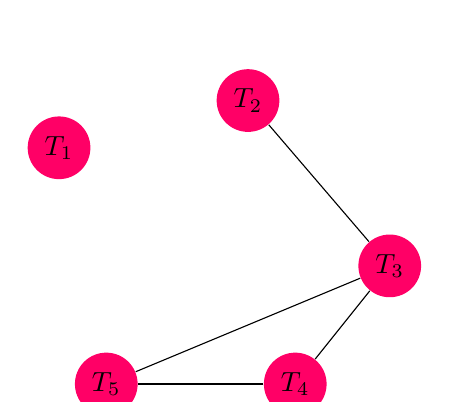
\begin{tikzpicture}[scale = 3]
		\node (a) at (0,1) [circle, fill = nicepink] {$T_1$};
		\node (b) at (0.8,1.2) [circle, fill = nicepink] {$T_2$};
		\node (c) at (1.4,0.5) [circle, fill = nicepink] {$T_3$};
		\node (d) at (1,0) [circle, fill = nicepink] {$T_4$};
		\node (e) at (0.2,0) [circle, fill = nicepink] {$T_5$};
		\draw (b) edge (c);
		\draw (c) edge (d);
		\draw (c) edge (e);
		\draw (d) edge (e);
		\end{tikzpicture}
	\end{center}
	\caption{A small network example}\label{toy_network}
\end{figure}

It is reasonable to use a pairwise RMF. It is also common to assume a log linear function \cite{machine_learning}. An initial guess could be
\[
\psi_{s\sim t} (y_s,y_t) = \exp(\b{\theta} \cdot \b{1}_{y_s = i,y_t = j})
\]
where $\theta = (0,\log(P(s)), \log(P(t)),\log(\nhalf(P(s|t) + P(t|s))))$. This makes sense when we have only unconnected nodes. It also also penalizes leaving out nodes that are connected to the nodes we do have. However, this penalizes very harshly if a hub node is included in $\b{y}$..

A small network example can be used to demonstrate possibilities. Consider the network shown in \cref{toy_network}. Assume that
\[
p(\b{x}) = \prod_{s\sim t} \psi_{st}(\b{x})\prod_{s}\psi_s(\b{x})
\]
To start, determine the distribution of an independent node ($T_1$). Clearly
\[
P(T_1 = x) = \psi_{1}(x)
\]
Similarly, we should have
\[
P(T_2 = x) = \psi_2(x) = \int \psi_2(x)\psi_{23}(y) dy =  \bE (P(T_2 = x|T_3))   
\]
One possibility is a binomial:
\[
P\left(T_1 = \frac{k}{N}\right) = \binom{N}{k}p^k(1-p)^{N-k}
\]
where $p$ is the proportion of times $T_1$ appears in the data, the sum of abundances of $T_1$ in the data divided by a scaling parameter $N$. But then, it's natural to take $N$ large and get a Gaussian by the CLT. This suggests a multivariate Gaussian as another possibility. Then
\[
\psi_{s\sim t}(\b{x}) = \exp\left(-\frac{1}{2} x_s \Lambda_{st}x_t\right)
\]
and
\[
\psi_s(\b{x}) = \exp\left(\eta_s x_s - \Lambda_{ss}x_s^2\right)
\]
\cite{machine_learning}. We already have the co-variance (normalized by the product of the standard deviations) matrix $\Sigma$, this is the adjacency matrix of our network. So, we have $\Lambda = \Sigma^{-1}$, and $\b{\eta} = \Sigma^{-1}\b{\mu}$. Unfortunately, $\Sigma$ is possibly singular, it's rank is bounded by the number of samples used to construct the network. This of course leaves us with no way to determine $\Lambda$. So, we have to try to approximate $\Lambda$ subject to the constraint that if $s \not\sim t$, $\Lambda_{st} = 0$. We can use the SVD:
\[
\Sigma = M S N^* \Rightarrow \Sigma^+ = N \tilde{S} M^*
\] 
where $\tilde{S}$ is diagonal with $1/s_i$ until you get to zero singular values, where you just put a $0$. Because $\Sigma$ is symmetric, we have $M^* = N$. Then,
\[
\Sigma^+ = N \tilde{S} N
\]
This is used, although it doesn't seem to preserve zeros. There's a function to do it in Scipy.

On the other hand, taking $N$ large and $p$ small we get an exponential random variable. So perhaps we could use
\[
\psi_1(x) = e^{-\lambda}\frac{\lambda^{Nx}}{(Nx)!}
\]
or more directly
\[
\psi_1(x) = \binom{N}{Nx}p^{Nx}(1-p)^{N-Nx}
\]
and using Stirling's formula,
\[
\log(\psi_1) \approx N\left[x \log\left(\frac{p}{x}\right) + (1-x)\log\left(\frac{1-p}{1-x}\right)\right]
\]

\subsection{Comparing configurations without specifying $\psi$}
To compare two configurations $\b{x}$ and $\b{y}$, we can inspect
\[
\frac{P(\b{x})}{P(\b{y})} > 1
\]
without knowing them. For that, I would need to identify which cliques change, and ask whether they increase or decrease. How exactly to decide that is a not totally clear. For a clique, we could assume that $\psi_c$ decreases if we have over half the nodes and reduce and still have at least half, but increase if the we have less than half and decrease. That is, let $c$ be a clique with $n$ members, and $\psi_c(k)$ be the value of $\psi_c$ with $k$ members ``on". Then
\[
\frac{\psi_c(k+1)}{\psi_c(k)}   \left\{\begin{array}{c c}
>1 & k>\nicefrac{n}{2}\\
<1 & k\leq \nicefrac{n}{2}
\end{array}\right.
\]
Then, we are asserting the cliques are most likely to either be all there or none there.

The algorithm for deciding which of two nodes should be on and which should be off would then be:
\begin{enumerate}[(i)]
	\item Identify cliques $c_1,...,c_m$ which contain one or both nodes
	\item compute $\frac{\psi_{c_i}(k^1)}{\psi_{c_i}(k^2)}$ for each  $i \in \{1,...,m\}$, where $k^j$ is the number of members present in configuration $j \in \{1,2\}$, and this fraction is computed according to a simple rule of the kind above.
	\item multiply these ratios: $\frac{P(\text{configuration 1})}{P(\text{configuration 2})} = \prod_{i=1}^k \frac{\psi_{c_i}(k^1)}{\psi_{c_i}(k^2)}$
\end{enumerate}

We need to specify that rule precisely. The simplest reasonable thing is linear
\[
\frac{\psi_c(k+1)}{\psi_c(k)} = \frac{2(1-r_{min})}{n - 1} k + r_{min}
\]
but one could imagine some kind of sigmoidal rule as well, so that around $\nicefrac{n}{2}$ this ratio is close to $1$. This makes sense on a $2$ clique, as it implies that
\[
\psi(2) > \psi(1) \; \& \; \psi(0) > \psi(1)
\]
and in general makes sense for $n$ even. It makes sense for $n$ odd as well. It asserts that it is equally likely to have on $\nicefrac{n}{2} \pm \nicefrac{1}{2}$. Finally, if we need to compare $k$ and $k+2$, we simply take
\[
\frac{\psi(k+2)}{\psi(k)} = \frac{\psi(k+2)}{\psi(k+1)}\frac{\psi(k+1)}{\psi(k)}
\]
That is, a discrete analogue to the chain rule.

To compare $P(v_1 =1 | \xi)$ and $P(v_2 = 1 | \xi)$, let $X$ be the configurations with $\xi$ and $v_1 = 1$, and $Y$ the configurations with $\xi$ and $v_2 = 1$. Then,
\[
P(v_1 = 1| \xi) = \sum_{x\in X} \frac{P(x)}{P(\xi)}
\]
and so
\[
P(v_1 = 1| \xi) > P(v_2 = 1|\xi) \Leftrightarrow \sum_{x\in X\setminus Y} P(x) >\sum_{y \in Y\setminus X} P(y)
\]
but inspecting $X$ and $Y$, we see that this is equivalent to 
\[
\sum_{x\in X\setminus Y} (P(x) - P(\tilde{x})) > 0
\]
where $\tilde{x} = x$ for all nodes except $v_1$ and $v_2$, while $x(v_1) = \tilde{x}(v_2) = 1$ and $x(v_2) = \tilde{x}(v_1) = 0$. This can be written
\begin{equation}
\sum_{x\in X\setminus Y}\prod_{c:v_1,v_2 \not \in c}\psi_c(x)\left(\prod_{c:v_1\text{ or }v_2  \in c}\psi(x) - \prod_{c:v_1\text{ or }v_2  \in c}\psi(\tilde{x}) \right) >0
\end{equation}
where $c$ are maximal cliques of the RMF.

In this way, we can compare two nodes. However, this does not give an easy way to compare sets of nodes.

\subsection{Diffusion based method.}
We would like to identify taxa likely to be present in a sample, given an initial estimate of abundances of taxa. Inspired by spectral clustering, I solve the diffusion equation on the graph in order to identify nodes that are likely present, given the sample data. The diffusion equation is
\[
\frac{\partial}{\partial t} u(v,t) = L u(v,t)
\]
where $v$ takes values in the vertex set of the graph. Then, we can encode ``known" information in three ways: initial values, boundary values, or a forcing vector.

\begin{inbox2}
	\begin{method}[Initial Value Problem]\label{initalCond}
		Let $u_i(t)$ be the solution at node $v_i$ to the discrete diffusion problem
		\[
		\frac{d}{dt}\b{u}(t)  = - L\b{u}
		\]
		where $L$ is the  graph Laplacian with initial conditions $u_i = 1$ if node $v_i$ is known to be ``on", $u_j = 0$ if $v_j$ is known to be ``off", and $u_k = 0.5$ (or $0$, or perhaps encoded with some confidence in $[0,1)$) if $v_k$ is unknown. I then normalize the initial vector so that it represents a probability distribution on the nodes.
		
		Then, if $\b{K}$ is the information ``known" and the values of $v_{k}$ and $v_{l}$ are unknown,
		\[
		\int_0^{\infty} u_k(t) dt - \int_0^{\infty} u_l(t) dt >  0 \Rightarrow  P(v_k=  1|\b{K}) > P(v_l = 1|\b{K})
		\]
	\end{method}
\end{inbox2}
These comparisons are easily computed. Solutions to the diffusion equation are of the form
\[
\b{u} = \sum_{i=1}^a c_i \b{1}|_{cc} + \sum_{i=a+1}^n c_i e^{-\lambda_i t} \b{\xi}_i 
\]
where $a$ is the number of connected components of the graph, and $\lambda_i,\b{\xi}_i$ are eigenvalue, eigenvector pairs of $L$. Note that each eigenvalue $\lambda_i \geq 0$, with $\lambda_i>0$ for $i = a+1,...,n$ \cite{vonLuxburg2007}. Then, assuming there is some initial mass on the connected component containing $v_1$ and $v_2$, 
\[
\int_0^{\infty} u_k(t) dt - \int_0^{\infty} u_l(t) dt =   \sum_{i=a+1}^n c_i  (\xi_{ki} - \xi_{li}) \int_0^{\infty} e^{-\lambda_i t} dt = \sum_{i=a+1}^n \frac{c_i}{\lambda_i}  (\xi_{li} - \xi_{ki}) 
\]
and $\b{c} = V^{-1}\b{u}(0)$. Therefore, it is straightforward to compute and compare the transitive terms of the solution:
\[
\int_0^{\infty}\left( u_k(t) - \sum_{i=1}^a c_i \right) dt = \sum_{i=a+1}^n \frac{c_i}{\lambda_i}\xi_{ki}
\]

We can regard this method as the Kolmogorov forward equation of a jump process that transitions from taxa to taxa which have an edge between them at a linear rate (see \cref{kfor}). The state space of this process is the affine space $\b{1}^{\perp} + \b{b}_1\cap \bZ^n_{\geq 0}$, where $\b{b}_i$ are the standard basis vectors. At any time $t$, $u_l(t)$ is the probability that the process is in the state $\b{e}_l$. This model clearly admits no extinction events and is complex balanced deficiency zero. In the deterministic setting, it has globally attracting equilibrium $\frac{1}{n}\b{1}$. Therefore, according to \cite{Anderson2010}, it has stationary distribution on each connected component
\[
\pi(\b{x}) = \frac{1}{Z_{cc}} \prod_{i=1}^n \frac{\left(\frac{1}{n}\right)^{x_i}}{x_i!}e^{-\frac{1}{n}}
\]
The state space of the system is $\{\b{b}_j\}$, and I note that for $j = 1,...,a$
\[
c_j = \pi(\b{b}_j) = \frac{1}{Z_{cc} n}e^{-\frac{1}{n}}
\]
and so the distribution is uniform on each connected component. If it is higher on one connected  component than an other, the above integral will be larger on that component. To compare within a connected component of the graph, I must look at the transient behavior, which I take by the integral above, subtracting this stationary distribution. This is going to allow us to compare nodes in the same connected component. I can then choose first the most likely connected components and then rank within those by transient behavior. 

Interestingly, I can regard this as the reaction network directly, deterministically modeled, which is the volume scaling limit of the jump process described above.

Note that if we give only one node initial mass, then the highest ranked (rank $0$) node is the node given the initial mass:

Let node $k$ be given initial mass, so $u(0) = \b{e}_k$. For any $l \neq k$, I show
\begin{equation}\label{first_wins}
\sum_{i =a+1}^n \frac{c_i}{\lambda_i}\xi_{ki} > \sum_{i =a+1}^n \frac{c_i}{\lambda_i}\xi_{li}
\end{equation}
I can diagonalize $L$ as $L = X\Lambda X^{-1}$. Let $\hat{L}$, $\hat{X}$, and $\hat{\Lambda}$ be the $n-a\times n-a$ matrices formed from $L$, $X$, and $\Lambda$ by taking rows \& columns corresponding to non-zero eigenvalues $\lambda_i$. Recall that $\b{c} = X^{-1}u(0) = (X^{-1})_k$, and because $L$ is symmetric I have $X^{-1} = X^T$. This implies that $c|_{\lambda >0} = \hat{X}^T_k$. Then, I have that
\begin{equation}
\sum_{i =a+1}^n \frac{c_i}{\lambda_i}\xi_{li} = (\hat{\Lambda}^{-1} \hat{X}^T_k)\cdot \hat{X}^T_l
\end{equation}
Furthermore, $X$ is a unitary matrix. This means that 
\begin{equation}
X^T_k \cdot X^T_l = \left\{\begin{array}{c c}
0 & k \neq l \\
1 & k = l
\end{array}\right.
\end{equation}
Furthermore, $ \hat{X}^T_k|_{\lambda = 0} \cdot \hat{X}^T_l|_{\lambda = 0} = \nicefrac{1}{n}$. Then,
\begin{equation}
\hat{X}^T_k \cdot \hat{X}^T_l = \left\{\begin{array}{c c}
-\nicefrac{1}{n} & k \neq l \\
1 - \nicefrac{1}{n} & k = l
\end{array}\right.
\end{equation}
Then, because $\hat{\Lambda}^{-1}$ is clearly positive definite, I can conclude that 
\begin{equation}
\sum_{i =a+1}^n \frac{c_i}{\lambda_i}\xi_{ki} = (\hat{\Lambda}^{-1} \hat{X}^T_k)\cdot \hat{X}^T_k > 0>   (\hat{\Lambda}^{-1} \hat{X}^T_k)\cdot \hat{X}^T_l = \sum_{i =a+1}^n \frac{c_i}{\lambda_i}\xi_{li} 
\end{equation}

This calculation reveals the nature of the relationship between this idea and spectral clustering. In spectral clustering, I ask about ``closeness" in the first $k$ eigenmodes of the diffusion process. Here, I ask a similar question, weighing the (transient) eigenmodes by their eigenvalue (and so rate of decay).

\begin{inbox2}
	\begin{method}[Boundary Value Problem]\label{boundarVal}
Let $u_i(t)$ be the solution at node $v_i$ to the discete diffusion problem
\[
\frac{d}{dt}\b{u}(t)  = - L\b{u}
\]
where $L$ is the  graph Laplacian with fixed values (which can be regarded as boundary values) $u_i = 1$ if node $v_i$ is known to be ``on", $u_j = 0$ if $v_j$ is known to be ``off". 

Then, if $\b{K}$ is the information ``known" and the values of $v_{k}$ and $v_{l}$ are unknown, and $\b{\tilde{u}}$ is the equilibrium solution to the diffusion problem,
\[
\tilde{u}_k dt >  \tilde{u}_l \Leftrightarrow  P(v_k=  1|\b{K}) > P(v_l = 1|\b{K})
\]
	\end{method}
\end{inbox2}

First, we establish conditions under which the boundary value version will always have an equilibrium. A ``boundary value" set on the graph is a set of fixed node values. We have seen already that the equilibrium of the diffusion problem is uniform, and so if we only have known ``on" nodes $\b{\tilde{u}} = \b{1}$.  If we specify off nodes as well, then there is not an equilibrium solution to the diffusion problem which gives those values at boundary nodes. However, this doesn't mean the boundary value problem (or, more precisely, the equivalent forced problem on the unknown subset) doesn't have an equilibrium solution. Take for example a complete graph on three nodes. If we prescribe one node as $1$ and one as $0$, the reduced problem is
\[
\frac{d}{dt} u = -2u + 1
\]
which has an equilibrium at $u = \nhalf$. This is not an equilirium to the entire problem, because in that case
\[
-L\begin{pmatrix}
1 \\ \nhalf \\ 0
\end{pmatrix} = \begin{pmatrix}
-2 & 1 & 1\\ 1 & -2 & 1 \\ 1 & 1 & -2
\end{pmatrix}\begin{pmatrix}
1 \\ \nhalf \\ 0
\end{pmatrix} = \begin{pmatrix}
-\nicefrac{3}{2} \\ 0 \\ \nicefrac{3}{2}
\end{pmatrix}
\]
The boundary value problem is equivalent to the forced problem on unknown nodes
\[
\frac{d}{dt}\b{u}|_{\b{U}} = L|_{\b{U}}\b{u} + f_{\b{K}}
\]
where $\b{u}|_{\b{U}}$ is the projection of $\b{u}$ onto the unknown set of nodes, $L|_{\b{U}}$ is $L$ with the rows and columns of the known nodes removed, and $f_{\b{K}}$ is the forcing due to the boundary conditions.
	
The nullity of $L$ is the number of connected components of the graph. Removing a column from a matrix will not lower the rank of that matrix if the column was a linear combination of other columns, which is the case precisely when the column is the first one removed that corresponds to some connected component of the graph. Therefore, as long as we specify at least one ``boundary value" from each connected component, $L|_{\b{U}}$ is non-singular and there exists a unique equilibrium to the boundary value problem.

The equilibrium is simply computed by solving 
\[
0 = L|_{\b{U}}\b{\tilde{u}} + f_{\b{K}}
\]

The boundary value problem can be interpreted as a population walking around the graph, with the population at some nodes maintained at fixed values. We then assume that probability that a node is ``on" is proportional to the size of the population at that node. Perhaps ``voters" are a good analogy. 

It can also be interpreted as the same reaction network as \cref{initalCond}, but the values of some species fixed.

\begin{inbox2}
\begin{method}[Forced Problem]\label{forcing}
Let $u_i(t)$ be the solution at node $v_i$ to the discrete diffusion problem
\[
\frac{d}{dt}\b{u}(t)  = - L\b{u} + f
\]
where $L$ is the  graph Laplacian and $f$ a forcing vector with $f_i = \alpha_{cc}$ if node $v_i$ is known to be ``on", $f_j = -\beta_{cc}$ if $v_j$ is known to be ``off", where $cc$ denotes a connected component of the graph. We choose $\alpha_{cc}$ and $\beta_{cc}$ so that on any connected component $cc$, $\sum \alpha_{cc}= \sum \beta_{cc}= 1$. 

Then, if $\b{K}$ is the information ``known" and the values of $v_{k}$ and $v_{l}$ are unknown, and $\b{\tilde{u}}$ is the equilibrium solution to the diffusion problem,
\[
\tilde{u}_k dt >  \tilde{u}_l \Leftrightarrow  P(v_k=  1|\b{K}) > P(v_l = 1|\b{K})
\]
\end{method}
\end{inbox2}

Notice that the kernel of $L$ is $\mathit{span}(\{\b{1}|_{cc}\})$, where $cc$ denotes a connected component of the graph. For an equilibrium solution to exist, any connected component with an ``on" node must also have an ``off" node, so that $f \in \mathit{span}(\{\b{1}|_{cc}\})^{\perp}$, which is the range of $L$ because $L$ is symmetric. 

We can easily compute the equilibrium solution by solving, as long as we have guaranteed that $f \in \mathit{range}(L)$. On a practical note, we use Numpy's least squares solver because the matrix $L$ is singular. Unfortunately, if we do not specify an off node in a connected component in which we do specify an on node (or vice versa), there is no equilibrium solution.

The third method can be interpreted much like \cref{boundarVal}. However, instead of the population being maintained at known nodes, we have a constant inflow or outflow from the graph at these nodes. 

This can also be regarded as the same chemical reaction network model as \cref{initalCond}, but now with inflow and outflow. 

\begin{figure}
	\begin{subfigure}[b]{0.5\linewidth}
			\begin{center}
			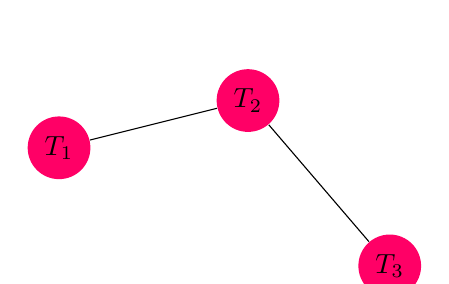
\begin{tikzpicture}[scale = 3]
			\node (a) at (0,1) [circle, fill = nicepink] {$T_1$};
			\node (b) at (0.8,1.2) [circle, fill = nicepink] {$T_2$};
			\node (c) at (1.4,0.5) [circle, fill = nicepink] {$T_3$};
			\draw (b) edge (c);
			\draw (a) edge (b);
			\end{tikzpicture}
		\end{center}
		\caption{A small network example}
	\end{subfigure}
	\begin{subfigure}[b]{0.5\linewidth}
		\begin{center}
			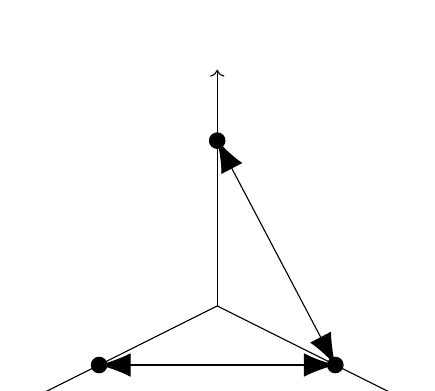
\begin{tikzpicture}[scale = 3]
				\draw[->] (0,0)--(0,1);
				\draw[->] (0,0)--(0.8,-0.4);
				\draw[->] (0,0)--(-0.8,-0.4);
				\fill (0,0.7) circle (1 pt);
				\fill (0.5,-0.25) circle (1 pt);
				\fill (-0.5,-0.25) circle (1 pt);
				\draw[{Latex[length=4mm]}-{Latex[length=4mm]}] (0,0.7) -- (0.5,-0.25);
				\draw[{Latex[length=4mm]}-{Latex[length=4mm]}] (0.5,-0.25) -- (-0.5,-0.25);
				\end{tikzpicture}
		\end{center}
	\caption{State transition graph for the IVP}
\end{subfigure}
\caption{Diffusion is equivalent to the Kolmogorov forward equations for the above system.}\label{kfor}
\end{figure}



\subsubsection{Tests of these methods}
I tested these three ideas on two small (unweighted) graphs, shown in \cref{tests}.

\begin{figure}
		\begin{subfigure}[b]{0.33\linewidth}
		\begin{center}
			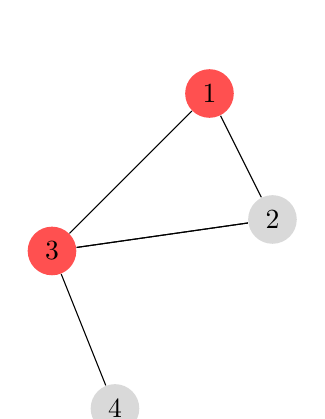
\begin{tikzpicture}[scale = 2]
			\node (a) at (1,2) [circle, fill = nicered] {$1$};
			\node (b) at (1.4,1.2) [circle, fill = lgray] {$2$};
			\node (c) at (0,1) [circle, fill = nicered] {$3$};
			\node (d) at (0.4,0) [circle, fill = lgray] {$4$};
			\draw (b) edge (c);
			\draw (a) edge (b);
			\draw (a) edge (c);
			\draw (b) edge (c);
			\draw (c) edge (d);
			\end{tikzpicture}
		\end{center}
		\caption{One tested configuration}
	\end{subfigure}
		\begin{subfigure}[b]{0.33\linewidth}
	\begin{center}
		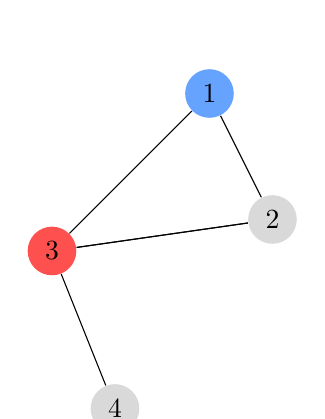
\begin{tikzpicture}[scale = 2]
		\node (a) at (1,2) [circle, fill = lblue] {$1$};
		\node (b) at (1.4,1.2) [circle, fill = lgray] {$2$};
		\node (c) at (0,1) [circle, fill = nicered] {$3$};
		\node (d) at (0.4,0) [circle, fill = lgray] {$4$};
		\draw (b) edge (c);
		\draw (a) edge (b);
		\draw (a) edge (c);
		\draw (b) edge (c);
		\draw (c) edge (d);
		\end{tikzpicture}
	\end{center}
	\caption{One tested configuration}
\end{subfigure}
	\begin{subfigure}[b]{0.33\linewidth}
		\begin{center}
			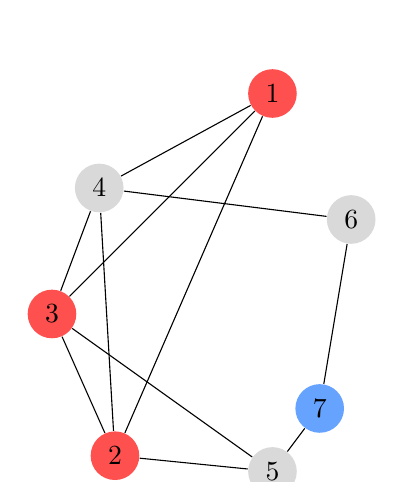
\begin{tikzpicture}[scale = 2]
			\node (a) at (1,2.3) [circle, fill = nicered] {$1$};
			\node (b) at (0,0) [circle, fill = nicered] {$2$};
			\node (c) at (-0.4,0.9) [circle, fill = nicered] {$3$};
			\node (d) at (-0.1,1.7) [circle, fill = lgray] {$4$};
			\node (e) at (1,-0.1) [circle, fill = lgray] {$5$};
			\node (f) at (1.5,1.5) [circle, fill = lgray] {$6$};
			\node (g) at (1.3,0.3)[circle, fill = lblue] {$7$};
			\draw (a) edge (b);
			\draw (a) edge (c);
			\draw (a) edge (d);
			\draw (b) edge (c);
			\draw (b) edge (d);
			\draw (c) edge (d);
			\draw (d) edge (f);
			\draw (f) edge (g);
			\draw (e) edge (g);
			\draw (c) edge (e);
			\draw (b) edge (e);
			\end{tikzpicture}
		\end{center}
		\caption{One tested configuration}
	\end{subfigure}
	\caption{Test networks. Gray nodes were ``unknown", blue nodes ``off", and red ``on".}\label{tests}
\end{figure}

\begin{table}
	\begin{center}
\begin{tabular}{|l|l|l|l|}
	\hline Configuration & Method & Ranking & Ties\\
	\hline
	\cref{tests}(a) &  IVP & 2, 4 & none  \\ \cline{2-4}
	 & BVP & 4, 2 & 4, 2 \\ \cline{2-4}
	 & Forcing & 2, 4 & none \\
	\hline
		\cref{tests}(b) &  IVP & 4, 2 &none \\ \cline{2-4}
	& BVP &4, 2 & none  \\ \cline{2-4}
	& Forcing &4, 2 & none\\
	\hline
		\cref{tests}(c) &  IVP & 4, 5, 6& none \\ \cline{2-4}
	& BVP & 4, 5, 6&  none\\ \cline{2-4}
	& Forcing &  4, 5, 6& none \\
	\hline
\end{tabular}
\end{center}
\caption{Results of ranking nodes by likelihood of being ``on" by the three above methods}\label{rankres}
\end{table}
	
I also tested these methods on a genus level network built from Pearson correlation higher than $0.8$ with $p < 0.05$ (determined by Monte Carlo simulation). This network had a number of connected components. I used a column of the sample data used to create the network as my configuration, with nodes with larger than mean abundance taken as ``on" and no abundance taken as ``off", while taxa with non-zero but below mean abundance taken as ``unknown". By analyzing all nodes using \cref{initalCond} (\cref{diffusion_sample} (a)), positive likelihood can be assigned to nodes assumed ``off" if they are connected to nodes assumed ``on". In the other two methods, only unknown and nodes assumed on can have positive likelihood (\cref{diffusion_sample} (b)).

\begin{figure}
	\begin{center}
	\begin{subfigure}[b]{0.48\linewidth}
	\begin{center}
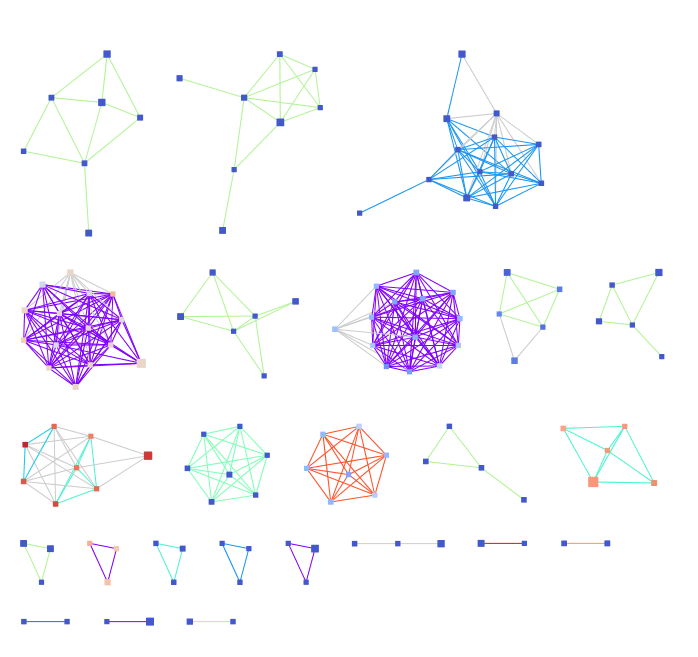
\includegraphics[scale = 0.3]{ranked_ivp.png}	
\end{center}
\caption{Result of \cref{initalCond}, with all nodes analyzed. Hotter colors indicate higher likelihood.}
\end{subfigure}
\begin{subfigure}[b]{0.48\linewidth}
		\begin{center}
		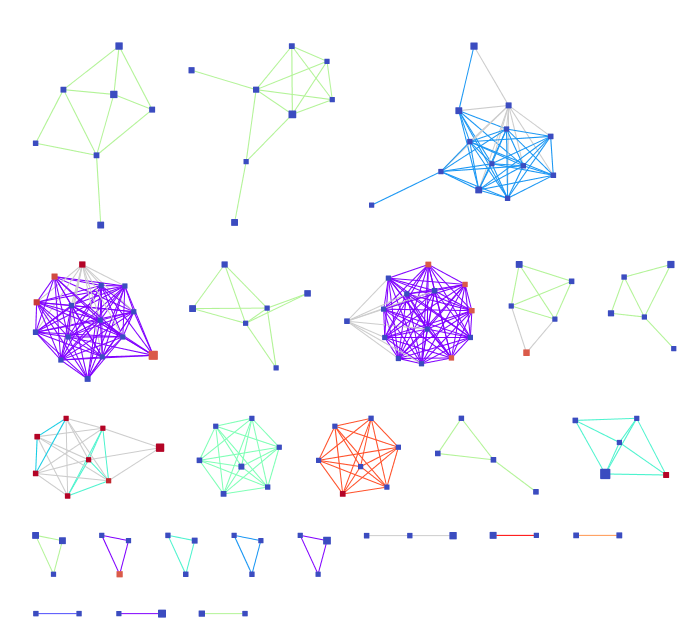
\includegraphics[scale = 0.3]{ranked_bdvp.png}	
	\end{center}
	\caption{Result of \cref{boundarVal}. Hotter colors indicate higher likelihood, with red indicating assumed ``on".}
\end{subfigure}
\begin{subfigure}[b]{0.48\linewidth}
		\begin{center}
		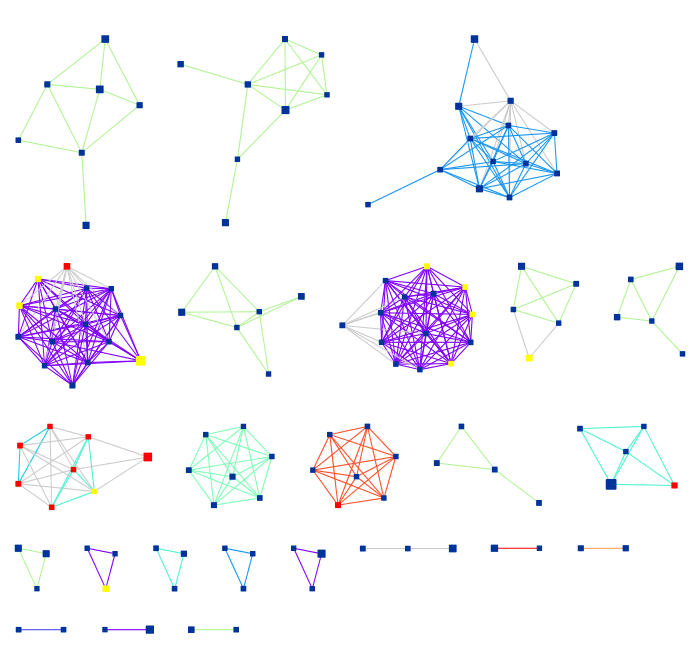
\includegraphics[scale = 0.3]{ranked_known_nodes.png}	
	\end{center}
	\caption{The ``known" set - blue is off and red is on, while yellow is unknown.}
\end{subfigure}
\caption{Result of diffusion methods. Edge color represents the shared sample type of the nodes (i.e. samply type the taxa was found most often in), with gray indicating different types.}\label{diffusion_sample}
\end{center}
\end{figure}	

We also tested \cref{initalCond} on networks built from over 1,300 samples and 300 test samples. We modified the test data by creating false positives and false negatives. Then, we ranked nodes in the modified test samples. We hope to see false negatives ranked highly and false positives ranked low.

\begin{figure}
	\begin{subfigure}{\textwidth}
\begin{center}
	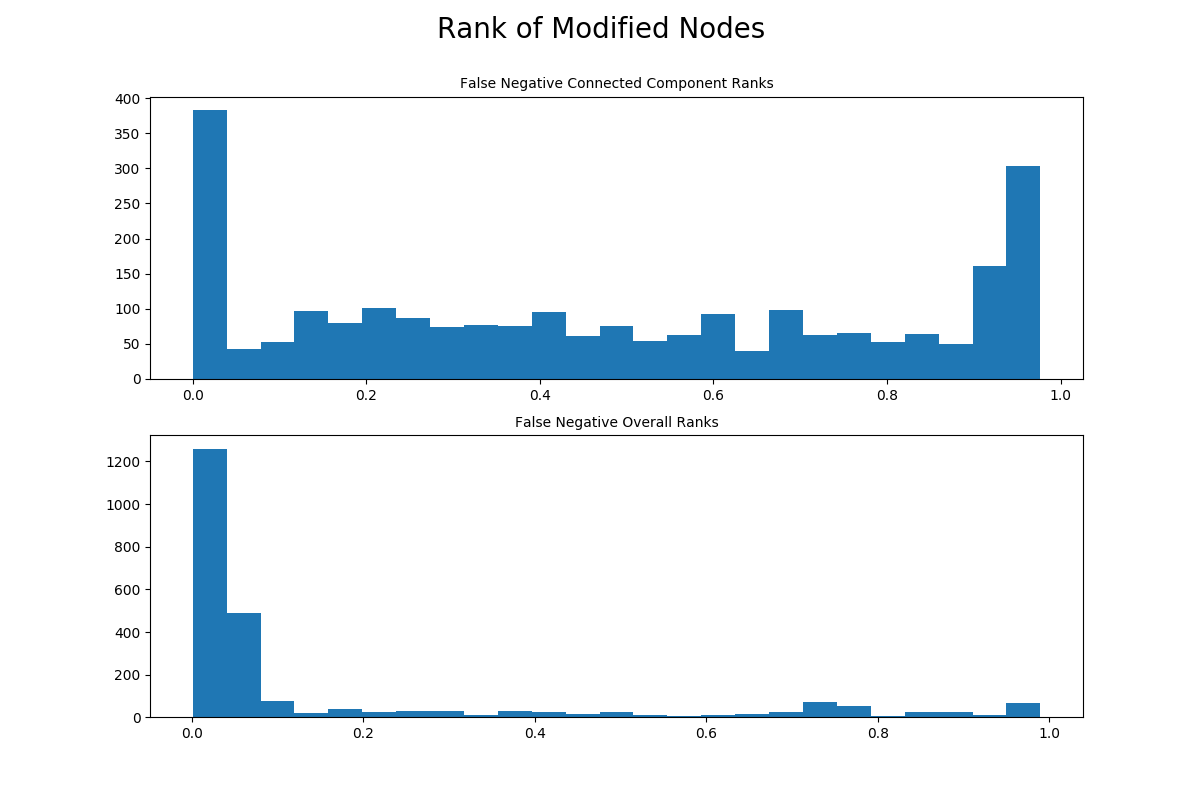
\includegraphics[scale = 0.5]{../stat_figs/merged2/species_rks_fn_full.png}
	\caption{Ranks of False Negatives on the network built from the entire data set.}
\end{center}
	\end{subfigure}
\caption{Diffusion Ranks}
\end{figure}

\section{Comparison of Networks}
We also may want to compare networks, especially networks produced from samples separated according to some category of metadata. There are of course the simple and obvious: size, radius, various connectivity and clustering metrics. There are also more interesting things, like the random walk kernel on graphs. Graph kernels are similar to an inner product on two graphs.

A graph kernel $k(G_1,G_2)$ must be symmetric and positive definite (an inner product must also be bilinear) \cite{Vishwanathan}. To compute the most common type (random walk kernels) we need to define the direct product of two graphs $G$ and $G'$. That is the graph $G_{\times}$ with vertices 
\[
(v_i,v_j') \in V \times V'
\]
and edges
\[
(v_i,v_j') \sim (v_k,v_l') \Leftrightarrow v_i \sim v_k \, \&\, v_j' \sim v_l'
\]
We can compute the adjacency matrix of this by computing the Kronecker product of the adjacency matrices of $G$ and $G'$. The Kronecker product of matrices $A$ and $B$ is
\[
A \otimes B = \begin{pmatrix}
a_{11} B & a_{12}B & \cdots & a_{1m}B\\
a_{21}B & \ddots & &\\
\vdots & & & \\
a_{n1}B & & & a_{nm}B
\end{pmatrix}
\]
A random walk on this graph is isomorphic to a random walk on either graph, and so one can consider a random walk on this graph as a simultaneous random walk on both. We can take the adjacency matrices normalized so row sums are 1, call those $A'$, $B'$, and then
\[
W_{\times}  = A' \otimes B'
\] 
This gives a stochastic matrix $W_{\times}$. Given distributions $p$ and $p'$, define $p_{\times}  = p \otimes p'$. Define the kernel
\[
k(G,G') = \sum_{k=0}^{\infty} \mu(k) q_{\times}^T W_{\times}^k p_{\times}
\]
where $q,q'$ are stopping probabilities, and $p,p'$ are initial distributions. This counts all the common random walks. The coefficients $\mu(k)$ serve two purposes. One is to make sure the sum is finite. The other allows one to tune the kernel to emphasize walks of certain lengths. I think it's called geometric if $\mu(k) = c^k$. However, this seems like it will overemphasize short walks, of which there will be many in common.


\subsection{Matching samples to networks}

Suppose we have different networks built from different types of data - i.e. healthy and unhealthy, or different regions, etc. We would like to match a sample with the network that makes most the sense. That is, we would like to say that a sample is more likely to be from one type of data than the other based on the network.

Clearly, the first pass is just asking how many taxa detected in the sample appear in each network. Next, we might ask how many clusters of a network are represented, or similarly how many taxa of the sample are in the same cluster in the network. The diffusion (\cref{initalCond}) idea can do something like this. We should see less nodes ranked highly that aren't in the sample if the sample ``fits" a network well. If we imagine a sample is created by performing a random walk on a graph and recording the nodes most often visited, the diffusion idea should identify nodes that the random walk ``should" have seen. If there are a bunch of those missing from the sample, we might think the network is not the right one. We could consider the map from rank to abundance, and integrate this against a kernel that weights towards the high ranks. As an example, let $\b{s}$ be the sample abundances (so $s_i$ is the abundance of organism $i$), and $\b{r}$ the ranking (so $r_i$ is the rank of organism $i$). We might take 
\[
F(\b{s},\b{r}) = \sum_{i=1}^n c^{r_i} s_i
\]
where $c<1$. Given a sample, we get ranking from a network $N_j$. Let $\b{r}^j(\b{s})$ be the ranking given by diffusion on network $j$. Then,
\[
F_j(\b{s}) = F(\b{s},\b{r}^j(\b{s})) = \sum_{i=1}^n c^{r_i^j} s_i
\]
and we can attempt to optimize over the networks we have (if there's only a few that's easy). The conjecture is then
\begin{conj}
	Assume that $F_j(\b{s}) > F_k(\b{s})$. Then $P(\b{s}|N_j) > P(\b{s}|N_k)$.
\end{conj}



Let's start with a very simple example. Consider the two networks shown in \cref{more_tests}. Using ``samples" $u_1 = (\nicefrac{1}{6},\nhalf,\nicefrac{1}{3},0,0,0)$, $u_2 = (\nicefrac{1}{6},\nhalf,0,0,\nicefrac{1}{3},0)$, and $u_3= (0,0,0,\nicefrac{1}{6},\nhalf,\nicefrac{1}{3})$ gave results shown in \cref{tiny_res}.


\begin{figure}
	\begin{subfigure}[b]{0.46\linewidth}
		\begin{center}
			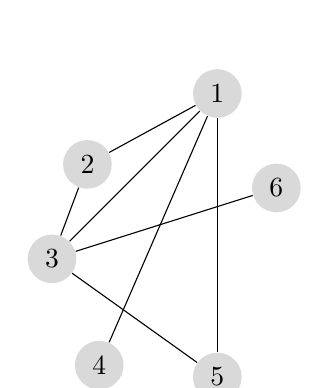
\begin{tikzpicture}[scale = 1.5]
			\node (a) at (1,2.3) [circle, fill = lgray] {$1$};
			\node (d) at (0,0) [circle, fill = lgray] {$4$};
			\node (c) at (-0.4,0.9) [circle, fill = lgray] {$3$};
			\node (b) at (-0.1,1.7) [circle, fill = lgray] {$2$};
			\node (e) at (1,-0.1) [circle, fill = lgray] {$5$};
			\node (f) at (1.5,1.5) [circle, fill = lgray] {$6$};
			\draw (a) edge (b);
			\draw (a) edge (c);
			\draw (b) edge (c);
			\draw (a) edge (d);
			\draw (a) edge (e);
			\draw (c) edge (f);
			\draw (c) edge (e);
			\end{tikzpicture}
		\end{center}
		\caption{Network $A_1$}
	\end{subfigure}
	\begin{subfigure}[b]{0.46\linewidth}
		\begin{center}
			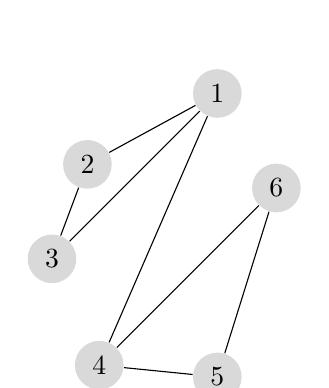
\begin{tikzpicture}[scale = 1.5]
			\node (a) at (1,2.3) [circle, fill = lgray] {$1$};
			\node (d) at (0,0) [circle, fill = lgray] {$4$};
			\node (c) at (-0.4,0.9) [circle, fill = lgray] {$3$};
			\node (b) at (-0.1,1.7) [circle, fill = lgray] {$2$};
			\node (e) at (1,-0.1) [circle, fill = lgray] {$5$};
			\node (f) at (1.5,1.5) [circle, fill = lgray] {$6$};
			\draw (a) edge (b);
			\draw (a) edge (c);
			\draw (b) edge (c);
			\draw (a) edge (d);
			\draw (e) edge (d);
			\draw (d) edge (f);
			\draw (f) edge (e);
			\end{tikzpicture}
		\end{center}
		\caption{Network $A_2$}
	\end{subfigure}
	\caption{Test networks. }\label{more_tests}
\end{figure}

\begin{figure}
	\begin{center}
	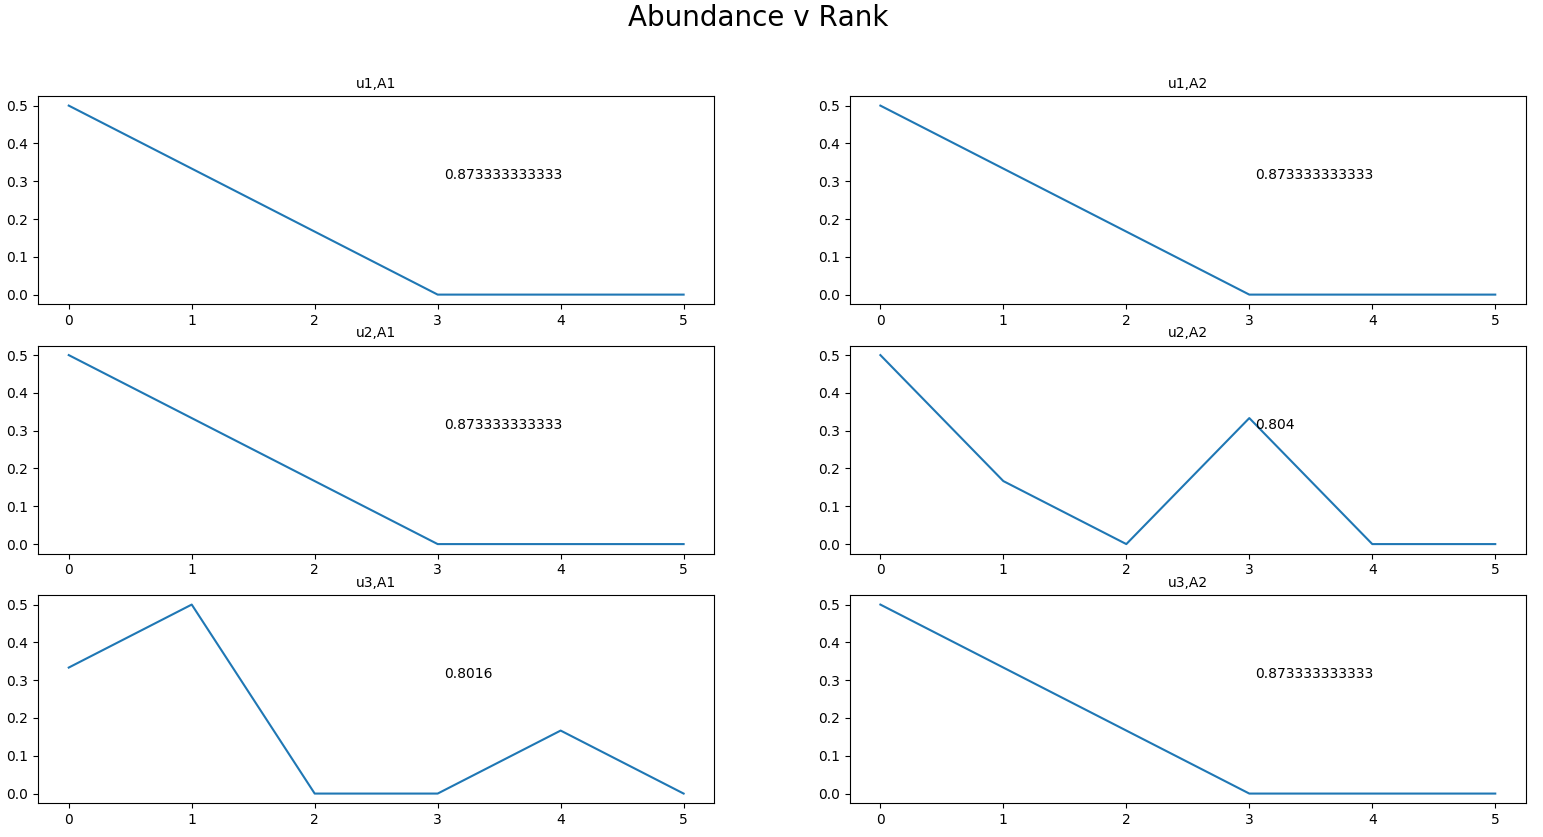
\includegraphics[scale = 0.4]{tiny.png}	
\end{center}
\caption{Results of sample assignment: $u_1$ cannot be decided, $u_2$ is assigned to network $A_1$, and $u_3$ is assigned to network $A_2$.}\label{tiny_res}
\end{figure}

I did the same on a column of training data for the species level network, a column of data that was held out of the network building, and a randomly generated sample. The results, shown in \cref{full_assign}, have the training data and held out data more likely to ``fit" the network than the random data.

\begin{figure}
	\begin{subfigure}[b]{0.9\linewidth}
	\begin{center}
	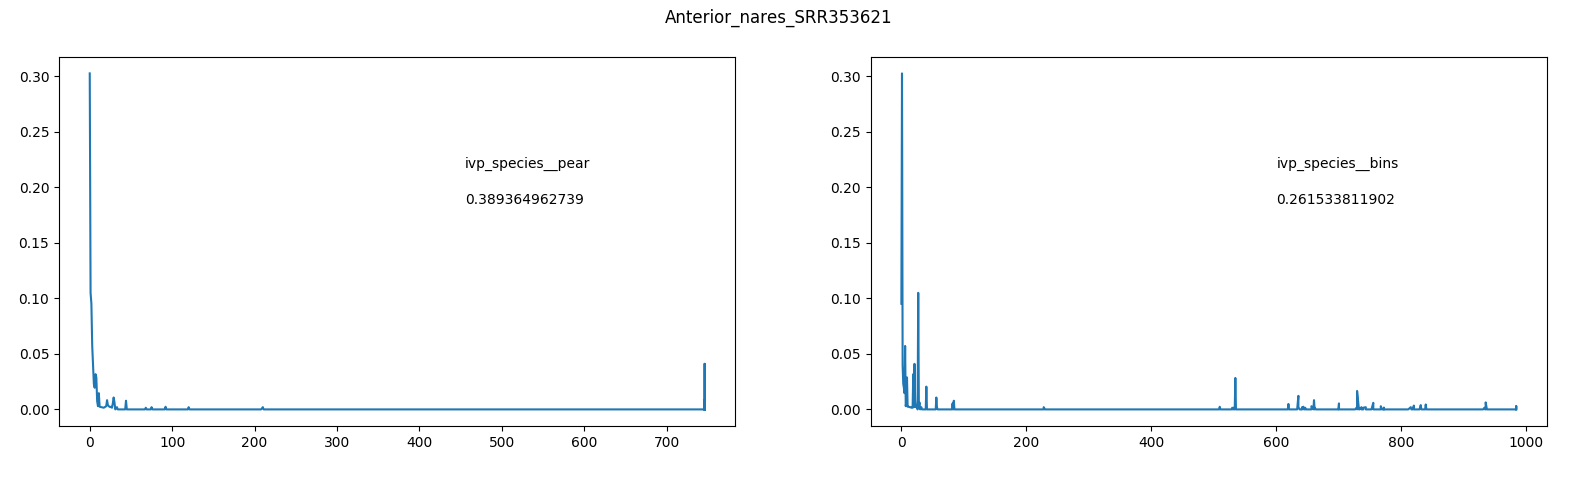
\includegraphics[scale = 0.45]{a_nares.png}	
	\end{center}
	\caption{Assignment of column of training data to networks built with binning (right) and with correlation (left).}
	\end{subfigure}
	\begin{subfigure}[b]{0.9\linewidth}
	\begin{center}
		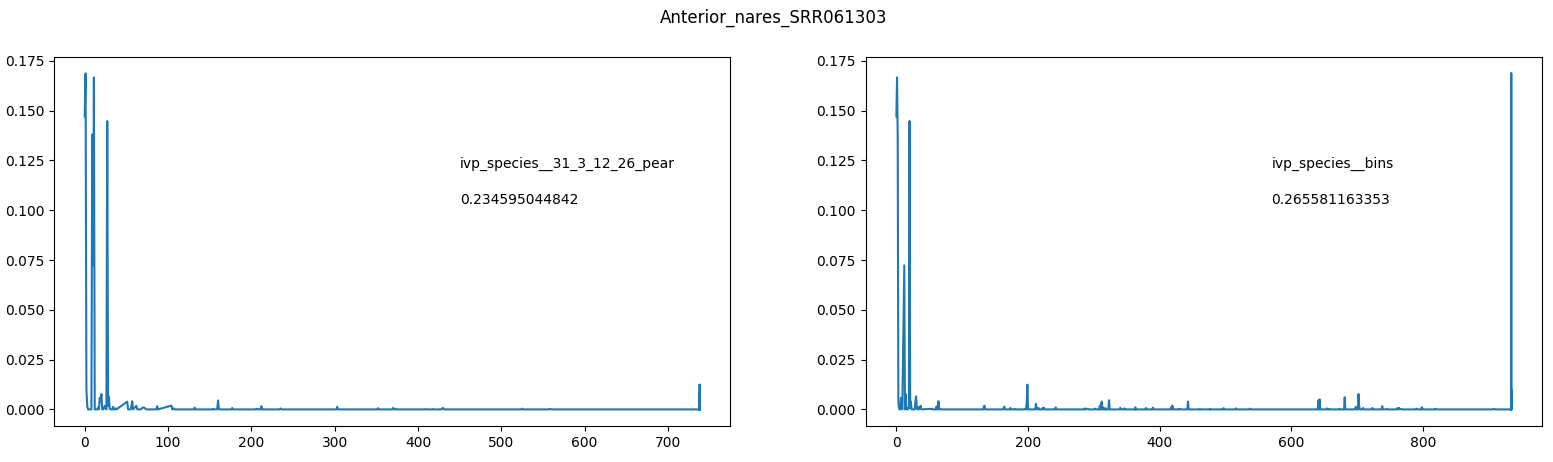
\includegraphics[scale = 0.45]{hldouts.png}	
	\end{center}
	\caption{Assignment of column of held out data to networks built with binning (right) and with correlation (left).}
\end{subfigure}
	\begin{subfigure}[b]{0.9\linewidth}
	\begin{center}
	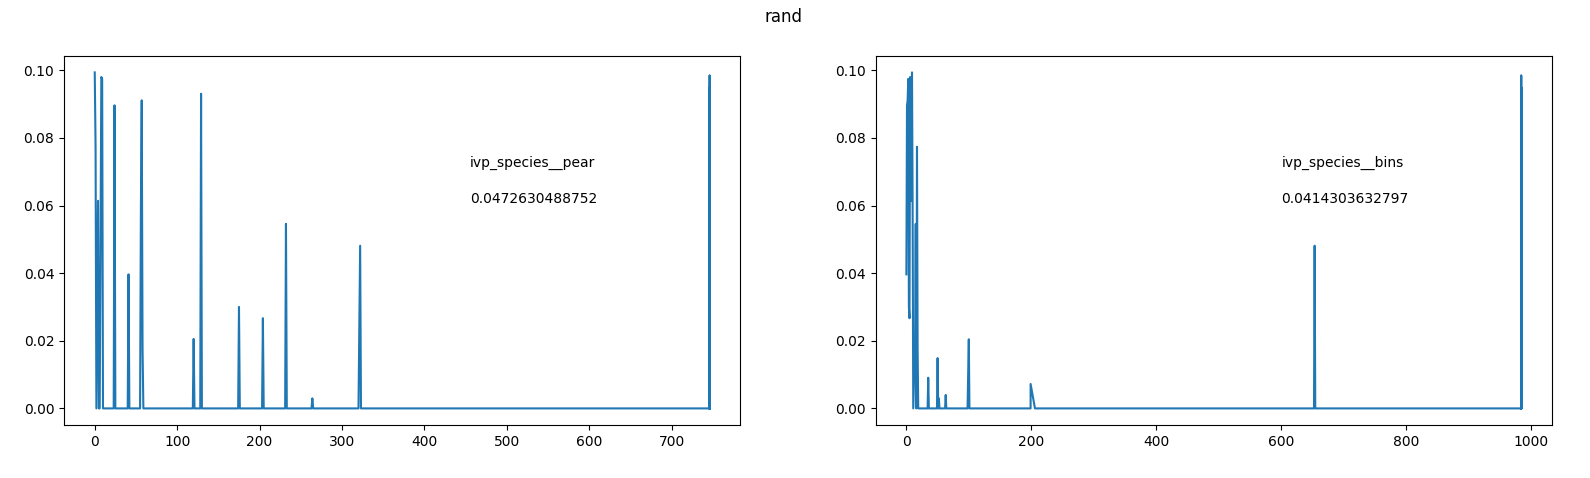
\includegraphics[scale = 0.45]{random.png}	
	\end{center}
	\caption{Assignment randomly generated data to networks built with binning (right) and with correlation (left). This random sample had 63 nodes chosen to be present, uniformly, and given an abundance drawn from a $unif[0,0.1]$ distribution.}
	\end{subfigure}
\caption{A training data column fits the network better than a randomly generated sample.}\label{full_assign}
\end{figure}

Formally, we have
\[
F_j(\b{s}) =\frac{1}{\|\b{s}\|} \sum_{i=0}^{n-1} c^i s_i
\]
where $\b{s} = (u_{j_1}(0),u_{j_2}(0),...,u_{j_n}(0))$ such that if 
\[
\frac{d}{dt}\b{u} = -L\b{u}
\]
and $U_l = \int_0^{\infty} u_l(t) dt$ then
\[
U_{j_1} \geq U_{j_2} \geq \cdots \geq U_{j_n}
\]

To test this idea, we construct networks using a data set of over 1,300 HMP samples and also subset of that network, determined by the sample location on the human body. We also had a set of 300 samples as testing data. For each network, we computed this fit for test samples which would have been used in the construction in that network, fit for test samples that would not have been used for construction of that network, and randomly generated samples, see \cref{fit_scores}.

\begin{figure}
	\begin{subfigure}{\textwidth}
	\begin{center}
	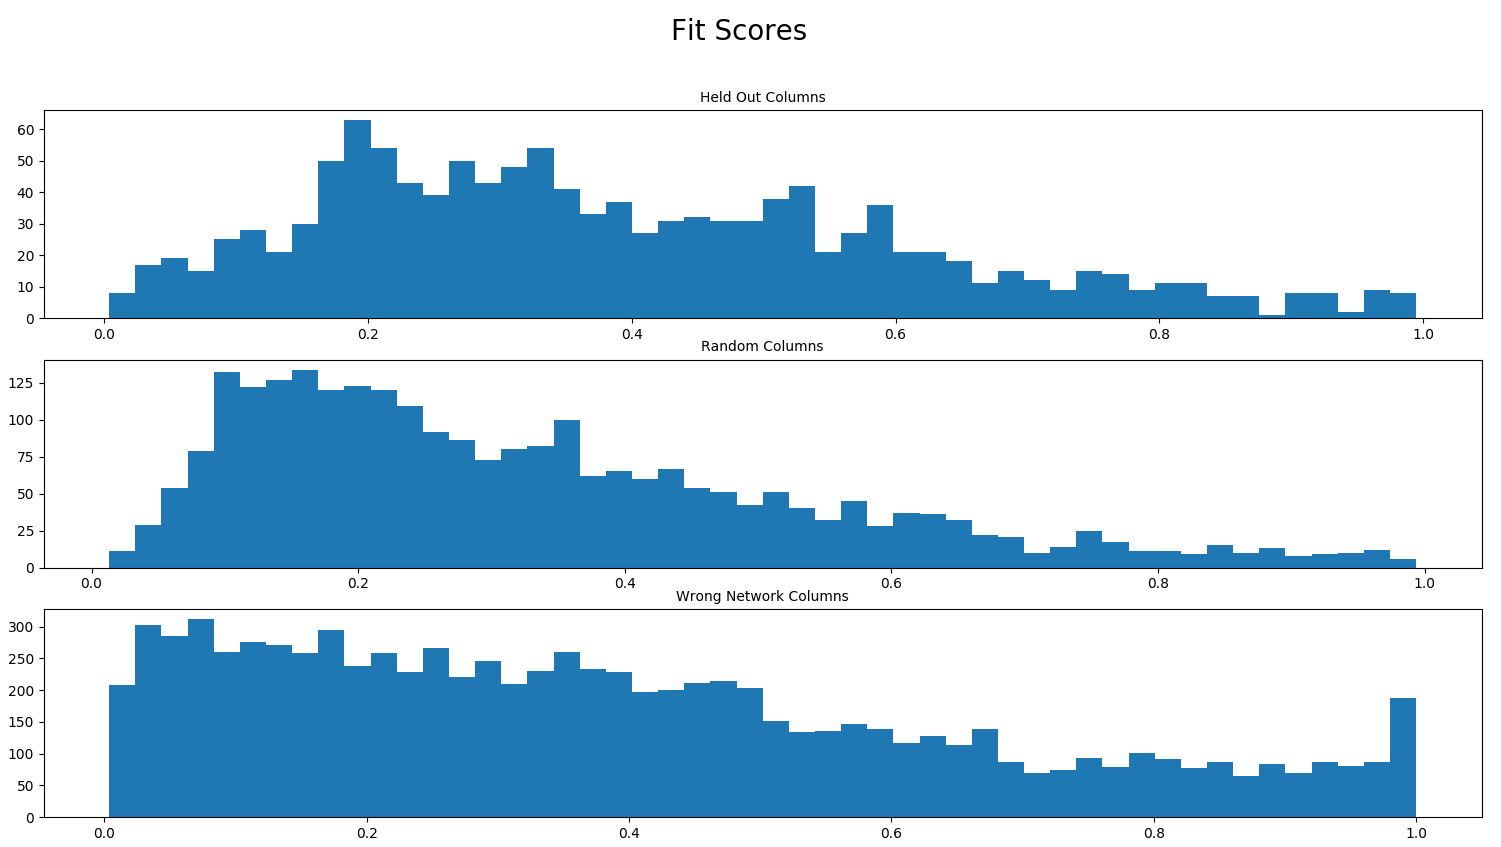
\includegraphics[scale = 0.4]{../stat_figs/merged2/species_fits_m2.png}
\end{center}
\caption{Fit scores of test samples (held out of network building) on all networks built (entire set and subsets of the data), fit of randomly generated samples, and fit of samples to networks that do not match their type.}
	\end{subfigure}
	\begin{subfigure}{\textwidth}
	\begin{center}
		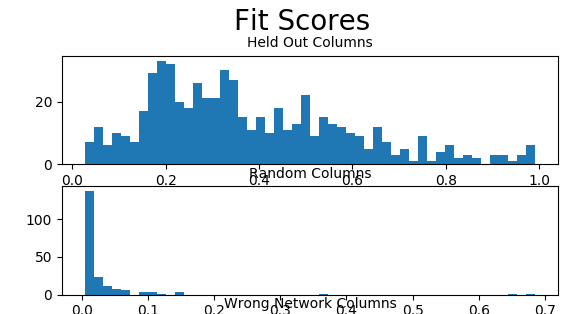
\includegraphics[scale = 0.5]{../stat_figs/merged2/species_fits_full.png}
	\end{center}
\caption{Fit scores of test samples (held out of network building) on the network built from the entire data set, and fit of randomly generated samples.}
\end{subfigure}
\caption{Fit scores for samples in networks. Random samples in (a) were samples in which 63 nodes were chosen to be present, uniformly, and given an abundance drawn from a $unif[0,0.1]$ distribution. In (b)'s random samples, I randomly choose the amount of non-zero values uniformly on the integers from 0 to the half a real sample length. I'll remake (a) like this. I'm redoing it all again with number of nonzero a Guassian with mean and std taken from the number of non-zero in the holdouts (nearest integer).}\label{fit_scores}
\end{figure}

\bibliographystyle{plain}
\bibliography{../../../summer17}
\end{document}